\section[Design]{Driftnode Design}

\subsection[Hardware]{Hardware}

\begin{figure}[h]
	\begin{center}
	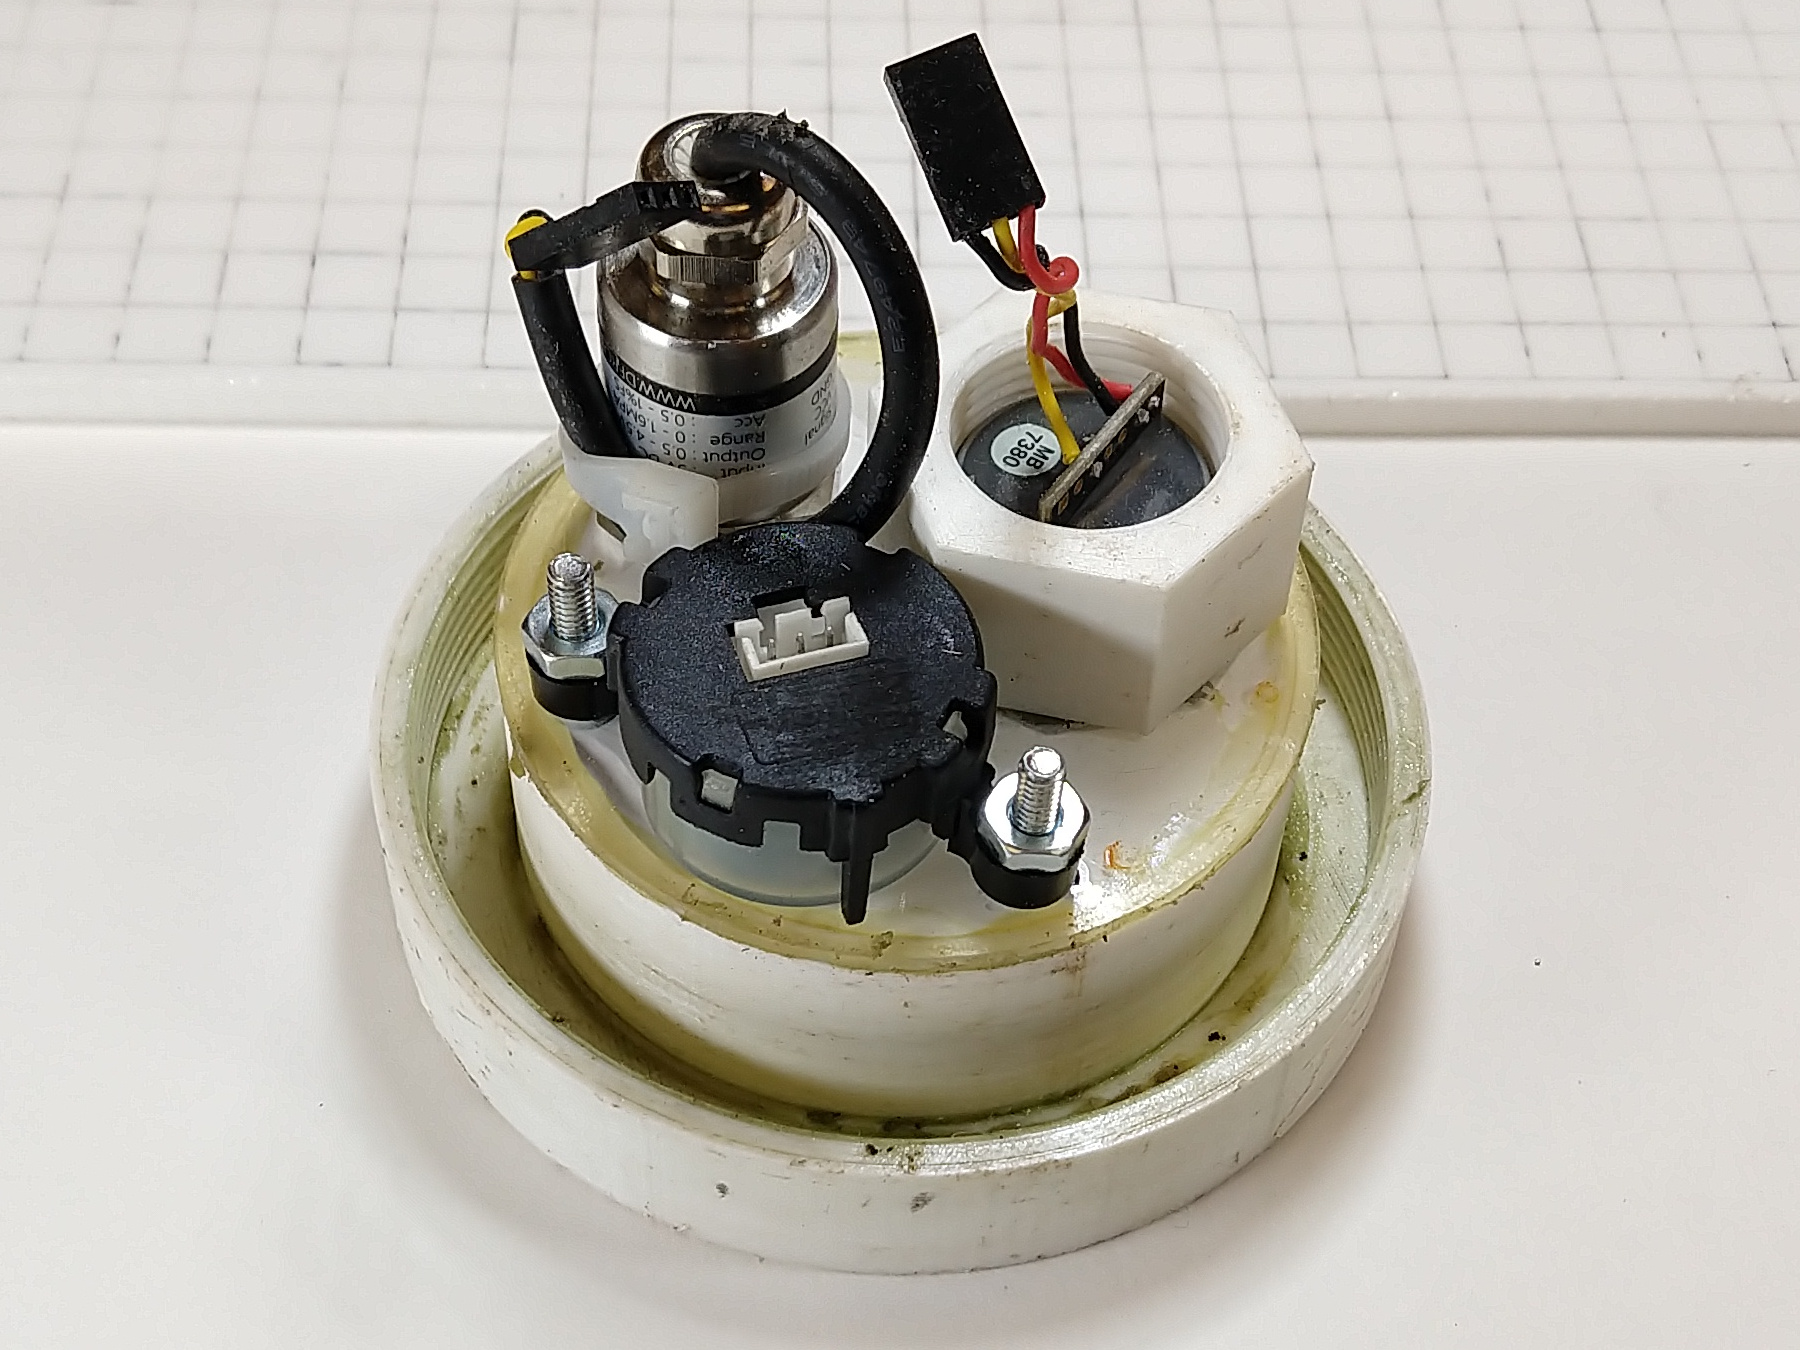
\includegraphics[width=.48\columnwidth]{driftnode/sensorcap.jpg}
	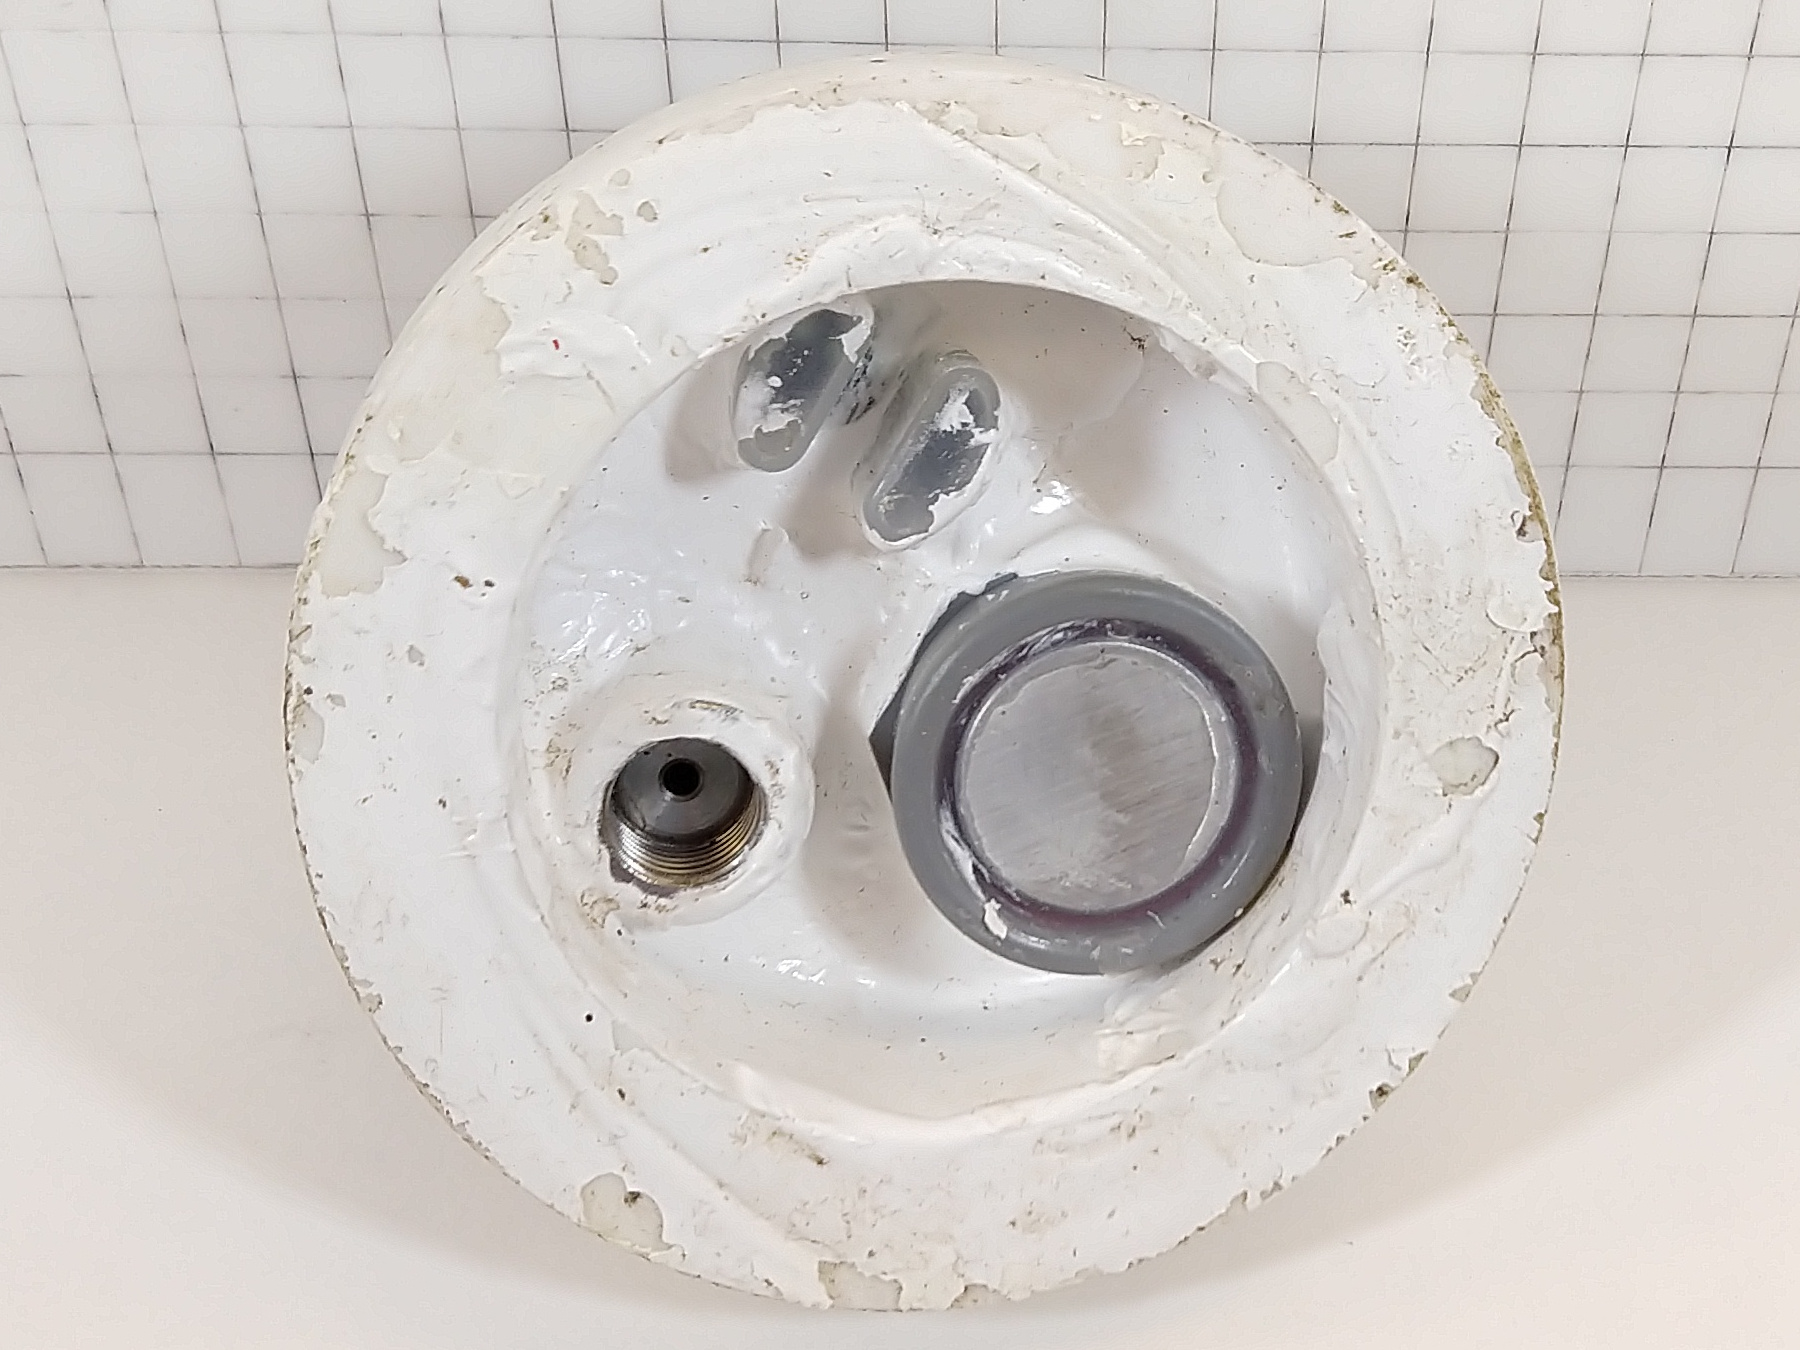
\includegraphics[width=.48\columnwidth]{driftnode/sensorcapbottom.jpg}
	\caption[Driftnode]{
		(Left) driftnode sensor cap. Threaded to the bottom of the driftnode. With turbidity, pressure and range sensor attached.
		(Right) bottom of driftnode sensor cap coated with rubber silicone.
	} \label{fig:sensorcap}
	\end{center}
	\vspace{-1em}
\end{figure}

You can see the driftnode's shell and electronics in Fig.~\ref{fig:driftnodeoverview}.
The current driftnode shell is an improvement upon the driftnode from \cite{drifterUSC}.
It is composed of a $\SI{43}{\centi\metre}$ PVC pipe, with 3D printed male threaded bushing glued to top and bottom of the pipe.
The glue joints and exterior surfaces of the male threaded bushing are coated with a rubber silicone coating for water proofing.
The driftnode's bottom and top caps can be threaded on to the threaded bushing on the pipe, completing the exterior of the drift node.
The bottom cap have sensors incorporated, after the sensors are installed, the exterior surfaces of the cap is cloated in the same rubber silicone coating as seen in Fig.~\ref{fig:sensorcap}.
The sensors used are all waterproof for their sensing elements.
The threaded sensor and top caps allow easy removal of the inside electronics and sensor for charging, debugging and improvement.

The driftnode's main electronics include a Raspberry Pi 3 embedded computer for logging sensor data and broadcasting the wireless access point.
The Raspberry Pi 3 is powered by a $\SI{10}{\ampere\hour}$ portable USB battery.
We used a proto-hat on the Raspbeery Pi to facilitate easy connection to sensors.

The driftnode can record its position with a commercially available GPS unit, in this case, it is the Adafruit Ultimate GPS Breakout board, connected to an extended GPS antenna.
The GPS sensor talks to the Raspberry Pi via serial communication.
We can record the orientation of the driftnode with a 9-axis intertial measurement unit sensor, in this case a Pololu MinIMU-9 v5.
We also have an analog turbidity sensor and pressure sensor for the driftnode, both output analog voltages, which is then converted to digital signal by the ADS1115 16-bit ADC board by Adafruit.
both the IMU and ADC board communicate to the Raspberry Pi through I$^{2}$C.

We have attempted to find a suitable underwater depth sensor.
We need a sensor that is small, preferably light weight, and relatively easy to interface.
However, many available depth sensor do not meet these requirements.
When speaking of underwater depth sensing via distance, fish finder sensor come to mind.
These sensor also output a point cloud similar to LIDAR sensor or depth cameras.
However, we have not been able to find a resource to interface with these sensor easily.
All commercially available fish finder sensor are coupled with either visualizer or communicate with proprietary visualizing software.
Another member of our lab is working on reverse engineering these sensors.
Fish finder are also typically larger than the area available in our sensor cap.
We have found two sensors, with compromise on accuracy.
One is the MB7380 by MaxSonar, which is a weatherproof sonar sensor that could be further water proofed then incorporated to our driftnode.
The second sensor is a JSN-SR04T based sonar sensor with a sonar probe connected by a water proof cable.
These two sensors were designed to be used in the air, with the waterproofing feature intended to make them more reliable outdoor.
However, we retro fitted them to work under water, taking into account that the speed of sound in water is $\SI{1498}{\metre/\second}$, four times faster than the speed of sound in air $\SI{343}{\metre/\second}$.

We left out the camera since our testing environment have very murky water.
Additionally, our extra turbidity, pressure and range sensor have taken up quite the entire area of the sensor cap.
Which can be added back in at a later date when we have a wider area for our sensor cap, or possibly a transparent tube which allow us to mount the camera facing to the side.

\subsection[Software]{Software}

The Raspberry Pi 3 is installed with embedded Linux operating system Raspbian.
Raspbian is based on Debian, which can run a simple version of the Robotics Operating System (ROS).
ROS allow us to connect multiple software nodes hosted on multiple computers.
This means we can easily connect one drift node to another, or a driftnode to a data collecting embedded computer carried on an AUV.

\begin{figure}[h]
	\begin{center}
	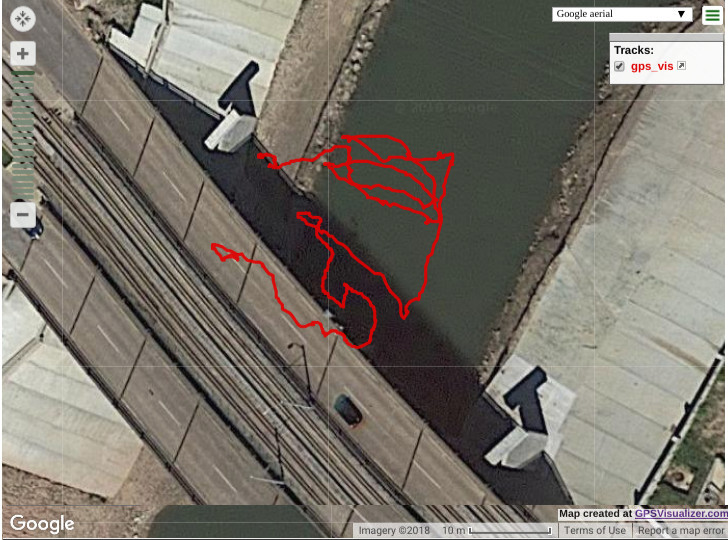
\includegraphics[width=0.48\columnwidth]{driftnode/dn2_gps_demo.jpg}
	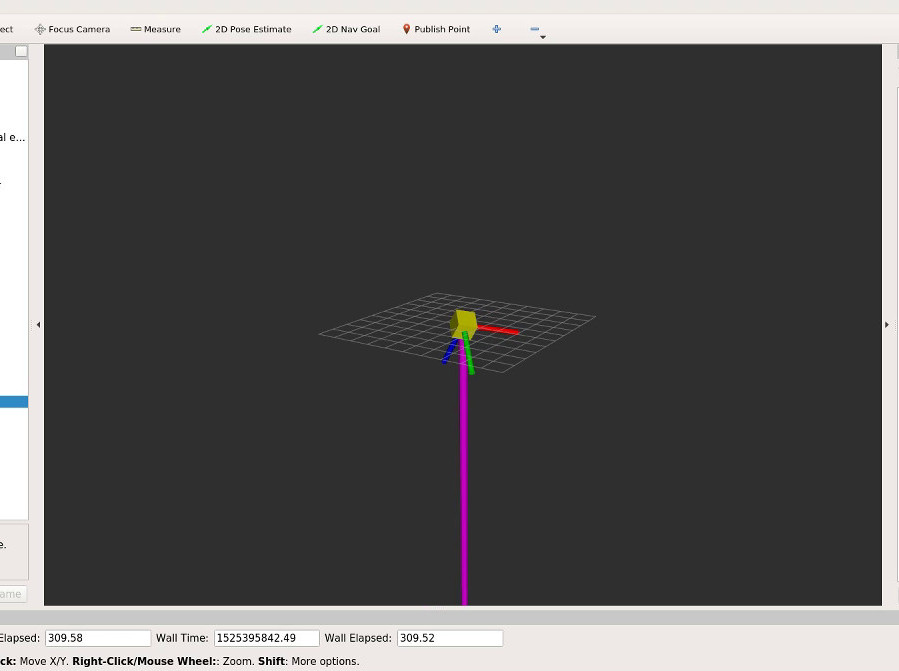
\includegraphics[width=0.48\columnwidth]{driftnode/dn2_imu_demo.jpg}
	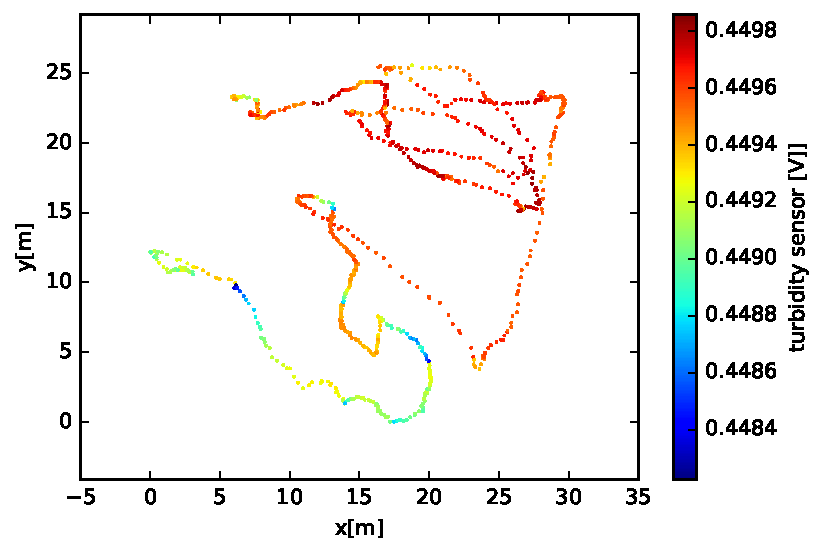
\includegraphics[width=0.48\columnwidth]{driftnode/dn2_turb.pdf}
	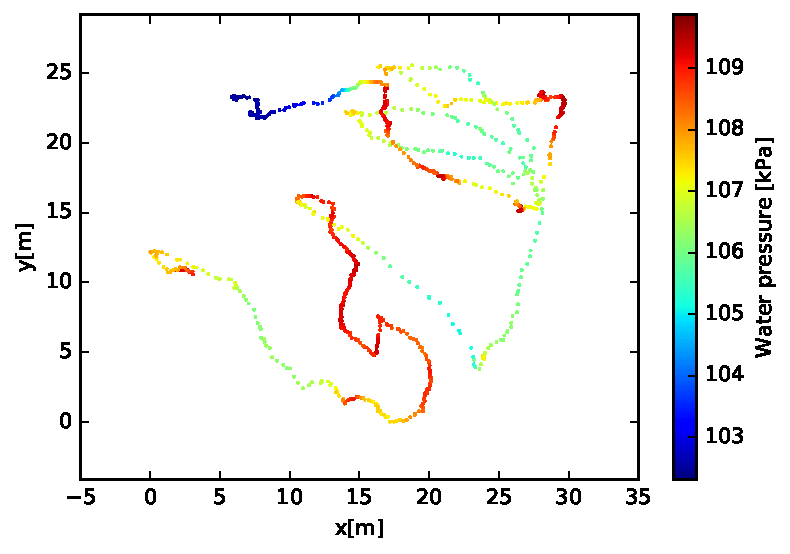
\includegraphics[width=0.48\columnwidth]{driftnode/dn2_press.pdf}
	\caption[Driftnode]{
		(Upper Left) GPS trace of a drift node mission.
		(Upper Right) IMU data visualized using Rviz, showing the orientation of the drift node.
		(Lower Left) Turbidity sensor data overlayed on top of the GPS trace.
		(Lower Right) Pressure sensor data overlayed on top of the GPS trace.
	} \label{fig:driftvis}
	\end{center}
	\vspace{-1em}
\end{figure}

All sensors are logged using ROS bag files.
Each sensor have its own Python script file that publishes on a topic for that sensor.
The GPS data is published with \textit{sensor\_msgs/NavSatFix} messages.
the IMU data is published with \textit{sensor\_msgs/IMU} messages.
The turbidity data is published with \textit{sensor\_msgs/Illuminance} messages.
The range data is published with \textit{sensor\_msgs/Range} messages.
The pressure data is published with \textit{sensor\_msgs/FluidPressure} messages.
ROS messages are recorded with publishing time and host name, so these messages can be played back synchronously.


Fig~\ref{fig:driftvis} shows visualizations for the GPS trace and the IMU data.
The GPS trace can be graphed by an online GPS visualizer, such as \emph{http://www.gpsvisualizer.com/}.
The IMU data is visualized to show the orientation of the drift node, using Rviz, a ROS tool.
The other data streams can be overlayed on to the GPS trace.
